% !TEX TS-program = pdflatex
% !TEX encoding = UTF-8 Unicode

% This is a simple template for a LaTeX document using the "article" class.
% See "book", "report", "letter" for other types of document.

\documentclass[11pt]{article} % use larger type; default would be 10pt

\usepackage[utf8]{inputenc} % set input encoding (not needed with XeLaTeX)

%%% Examples of Article customizations
% These packages are optional, depending whether you want the features they provide.
% See the LaTeX Companion or other references for full information.

%%% PAGE DIMENSIONS
\usepackage{geometry} % to change the page dimensions
\geometry{a4paper} % or letterpaper (US) or a5paper or....
% \geometry{margin=2in} % for example, change the margins to 2 inches all round
% \geometry{landscape} % set up the page for landscape
%   read geometry.pdf for detailed page layout information

\usepackage{graphicx} % support the \includegraphics command and options

% \usepackage[parfill]{parskip} % Activate to begin paragraphs with an empty line rather than an indent

%%% PACKAGES

\usepackage{setspace}
\usepackage{listings}
\usepackage{hyperref}
\usepackage{color}

\definecolor{dkgreen}{rgb}{0,0.6,0}
\definecolor{gray}{rgb}{0.5,0.5,0.5}
\definecolor{mauve}{rgb}{0.58,0,0.82}

\lstset{frame=tb,
  language=Python,
  aboveskip=3mm,
  belowskip=3mm,
  showstringspaces=false,
  columns=flexible,
  basicstyle={\small\ttfamily},
  numbers=none,
  numberstyle=\tiny\color{gray},
  keywordstyle=\color{blue},
  commentstyle=\color{dkgreen},
  stringstyle=\color{mauve},
  breaklines=true,
  breakatwhitespace=true,
  tabsize=3
}

\usepackage{booktabs} % for much better looking tables
\usepackage{array} % for better arrays (eg matrices) in maths
\usepackage{paralist} % very flexible & customisable lists (eg. enumerate/itemize, etc.)
\usepackage{verbatim} % adds environment for commenting out blocks of text & for better verbatim
\usepackage{subfig} % make it possible to include more than one captioned figure/table in a single float
% These packages are all incorporated in the memoir class to one degree or another...

%%% HEADERS & FOOTERS
\usepackage{fancyhdr} % This should be set AFTER setting up the page geometry
\pagestyle{fancy} % options: empty , plain , fancy
\renewcommand{\headrulewidth}{0pt} % customise the layout...
\lhead{}\chead{}\rhead{}
\lfoot{}\cfoot{\thepage}\rfoot{}

%%% SECTION TITLE APPEARANCE
\usepackage{sectsty}
\allsectionsfont{\sffamily\mdseries\upshape} % (See the fntguide.pdf for font help)
% (This matches ConTeXt defaults)

%%% ToC (table of contents) APPEARANCE
\usepackage[nottoc,notlof,notlot]{tocbibind} % Put the bibliography in the ToC
\usepackage[titles,subfigure]{tocloft} % Alter the style of the Table of Contents
\renewcommand{\cftsecfont}{\rmfamily\mdseries\upshape}
\renewcommand{\cftsecpagefont}{\rmfamily\mdseries\upshape} % No bold!

%%% END Article customizations

%%% The "real" document content comes below...

\title{Accidental Deaths and Injuries Data Analasys}
\author{Anja Miletić, Mateja Marjanović}
%\date{} % Activate to display a given date or no date (if empty),
         % otherwise the current date is printed 

\begin{document}
\pagenumbering{gobble}
\maketitle
\newpage

\doublespacing
\tableofcontents
\singlespacing
\newpage

\pagenumbering{arabic}

\section{Uvod}
Podaci su skinuti na linku \url{http://www.gunviolencearchive.org/reports}. Podaci se nalaze u dve datoteke: deaths.csv i injuries.csv i predstavljaju izvestaje o 
slucajnim povredama i smrtnim slucajevima nastalim koriscenjem vatrenog oruzja u Sjedinjenim Americkim Drzavama. 

\section{Analiza i pretprocesiranje podataka}
Obe datoteke sadrze tabele sa istim kolonama. Opisi kolona su dati u tabeli 1.
\newline\newline
\begin{tabular}{|l|l|}
\hline
Incident Date & datum incidenta u obliku Mesec dan, godina \\
\hline
State & savezna americka drzava u kojoj se dogodio incident \\
\hline
City or County & grad ili okrug u kome se dogodio incident \\
\hline
Adress & adresa na kojoj se dogodio incident \\
\hline
\# Killed & broj ubijenih osoba \\
\hline
\# Injured & broj povredjenih osoba \\
\hline
\end{tabular}

\subsection{Analiza podataka}
Kolonu koja predstavlja adrese cemo u nastavku ignorisati. 
\begin{lstlisting}
#remove column Adress
df = df[['Incident Date','State','City Or County','# Killed','# Injured']]
\end{lstlisting}

	
	
	\newpage
	\section{Klasterovanje}
	Proces klasterovanja izvrsen je na podacima koji su pre samog izvrsavanja pripremljeni (pretprocesiranje i namestanje podataka). 
	Podaci koji su prosledjeni imaju dva atributa, to su 'State' i 'Number of Incidents', 'State' predstavlja drzavu, a 'Number of Incidents' predstavlja 
	ukupan broj incidenata (slucajnih povreda i slucajnih ubistava) u toj drzavi.
	
	\subsection{Pripremanje podataka za klasterovanje}
	Da bismo izvrsili klasterovanje koje ima smisla, gde moze da se vidi koji podaci su slicniji, a koji razlicitiji, moramo da prvo te podatke izmenimo na 
	neki nacin i namestimo ih da budu takvi da nam odgovaraju. U narednom kodu napisanom u Python-u smo izmenili podatke iz 
	processed\_deaths.csv i processed\_injuries.csv i napravili novi fajl summedIncidentsPerState.csv.
	\newline
	
	\begin{lstlisting}
def changeDateFormat(df):
	for i, row in df.iterrows():
		month = row["Incident Date"].strip().split(' ')[0].split(',')[0]
		df.set_value(i, "Incident Date", month)
	
	df = df.drop(columns = ["Unnamed: 0", "Incident Date", "City Or County"])
	
	allIncidents = {}
	allStates = []
	for i, row in df.iterrows():
		state = row["State"].strip()
		if state not in allStates:
			allStates.append(state)
			allIncidents[state] = int(row["# Injured"]) + int(row["# Killed"])
		else:
			allIncidents[state] += int(row["# Injured"]) + int(row["# Killed"])
		df = df.drop([i])
	
	df = df.drop(columns = ["# Killed", "# Injured"])
	for k, v in allIncidents.iteritems():
		state = k
		numberOfDeaths = v
		df = df.append({"State" : state, "# Incidents" : int(numberOfDeaths)}, ignore_index = True)
	
	return df
	
    \end{lstlisting}
	
	\subsection{Prosledjivanje generisanih podataka i klasterovanje}
	Sad kad smo generisali podatke koristimo ih u Knime-u.
	Prvo citamo podatke sa CSV Reader-om, zatim ih saljemo na normalizaciju, tj. da se vrednosti iz kolone sa brojem ubistava skaliraju na interval [0, 1].
	Posle toga racunamo Euklidska rastojanja podataka, pa ta rastojanja i izlaz iz cvora koji je normalizovao podatke saljemo DBSCAN cvoru koji 
	dodaje jos jednu kolonu i svakoj instanci dodeljuje neku vrednost u zavisnosti od toga gde se nalazi.
	Ostalo je samo jos da se iscrtaju podaci, da bismo to uradili koristimo Color Manager i Scatter Plot.
	\newline
	
	\begin{figure}[h!]
	\centering
		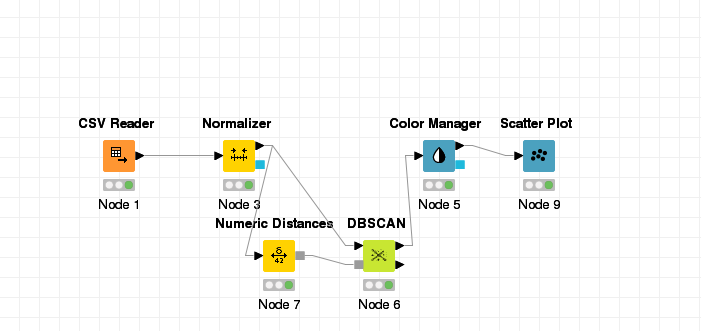
\includegraphics[width=0.8\textwidth]{klasterovanjeKnime}
		\caption{Izgled klasterovanja podataka u Knime-u}
	\end{figure}
	
	
	\newpage
	\subsection{Izgled klasterovanih podataka i analiza}
	Sada imamo podatke koji su podeljeni, svaki pripada nekom klasteru (neki pripadaju klasteru Noise) i svakom klasteru je dodeljena druga boja. Moze se 
	primetiti da je drzava u kojima ima vise ubistava mnogo manje nego drzava u kojima ima imanje. Npr. u Teksasu ima toliko vise nego bilo gde drugde da se 
	Teksas dozivljava kao sum.
	
	\begin{figure}[h!]
	\centering
		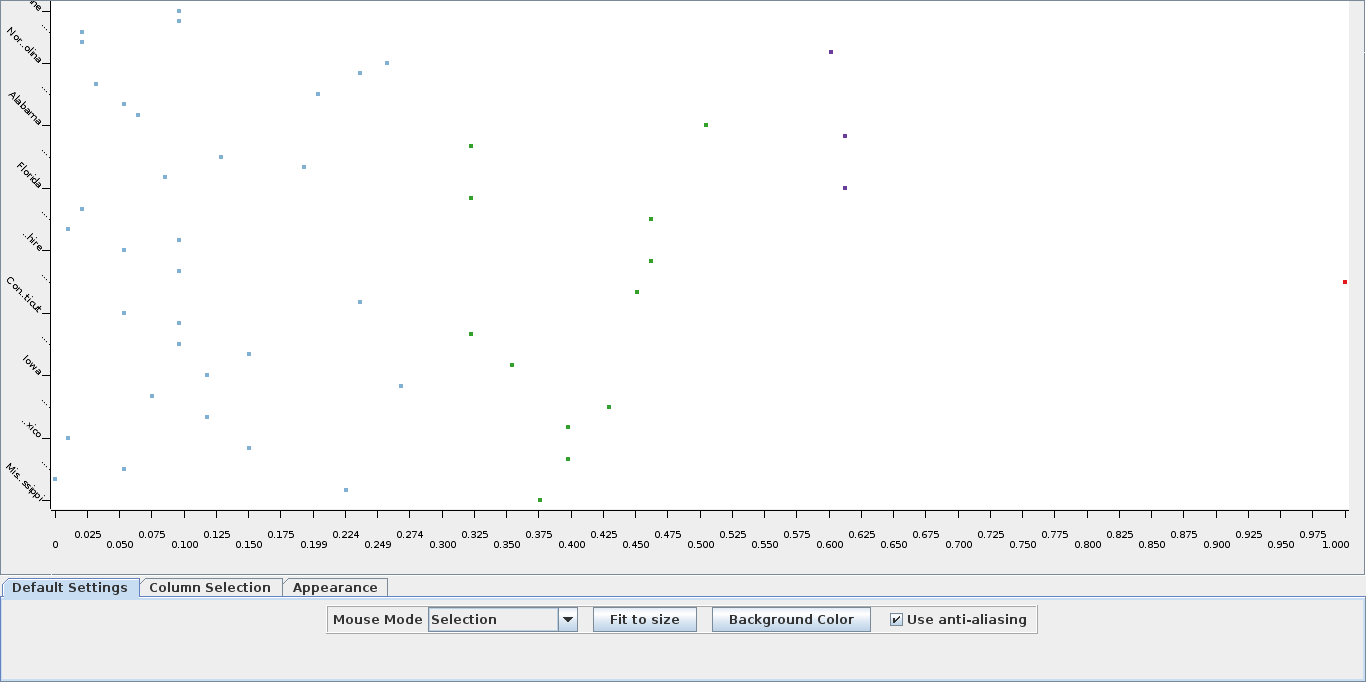
\includegraphics[width=0.8\textwidth]{klasterovanje1}
		\caption{Klasterovani podaci koji prikazuju zavisnost drzave i broja ubistava u toj drzavi}
	\end{figure}
	
	\newpage
	\section{Klasifikacija}
	Proces klasifikacije ili nadgledanog ucenja slicno kao i klasterovanje izvrsavamo na podacima koje smo generisali u drugom programu, zatim smo u 
	Knime-u te podatke iskoristili i izvrsili klasifikaciju. 
	Uradjene su dve klasifikacije. 
	Jedna je predvidjanje da li ce u odredjenom danu u nedelji u odredjenom mesecu biti malo, srednje ili puno incidenata. 
	Malo incidenata znaci da se u tom mesecu, u tom danu u nedelji (npr. svakom ponedeljku) ukupno desilo manje od 8, srednje znaci da je taj broj izmedju 8 i 15, 
	a puno vise od 15. Sa ovim brojevima ima slican broj parova (dan u nedelji, mesec) (blizu 33\% svako). To nije slucajnost, s obzirom na to da je 
	uzoracka sredina broja ubistava 12.8.
	U drugoj klasifikaciji izvrsava se predvidjanje da li ce biti puno (vise od 1) ili malo (manje jednako 1) incidenata u nekoj drzavi u nekom gradu.
	
	\subsection{Klasifikacija: Dan u nedelji, mesec, broj incidenata}
	Kao i ranije prvo podatke zelimo da transformisemo i dobijemo zeljeni oblik. U ovom slucaju zeljeni oblik bi bio da imamo kolonu mesec, dan u nedelji i 
	ukupan broj incidenata u toj kombinaciji (meseca i dana u nedelji). Sledeci kod ce generisati novi fajl u kome ce se nalaziti podaci.

	\begin{lstlisting}
def changeDateFormat(df):
	df = df.drop(columns = ["Unnamed: 0", "Incident Date"])
	
	incidents = {}
	for i, row in df.iterrows():
		state = row["State"].strip()
		city = row["City Or County"].strip()
		if state + ":" + city not in incidents:
			incidents[state + ":" + city] = int(row["# Injured"]) + int(row["# Killed"])
		else:
			incidents[state + ":" + city] += int(row["# Injured"]) + int(row["# Killed"])
		df = df.drop([i])
	
	df = df.drop(columns = ["# Killed", "# Injured"])
	for k, v in incidents.iteritems():
		key = k.split(':')
		city = key[1]
		state = key[0]
		numberOfDeaths = v
		df = df.append({"State" : state, "City Or County" : city, "# Incidents" : int(numberOfDeaths)}, ignore_index = True)
	
	return df
	\end{lstlisting}
	
\end{document}






























